% 0436(본책 79쪽) — 원 위 네 점 A·B·C·D, AB·CD 의 연장선의 교점 P(위), AC·BD 의 교점 Q, ∠P=30°, ∠BQC=70°, ∠BDC=x. 답(x)은 적지 않는다. 스캔 삽화를 TikZ 로 다시 그림.
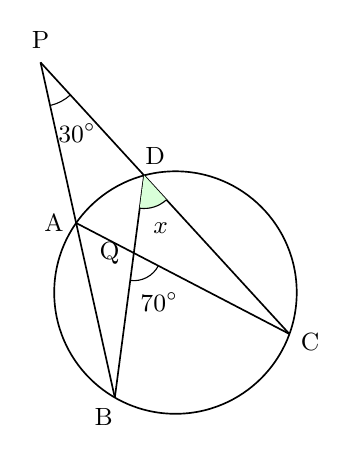
\begin{tikzpicture}[scale=1.4, line width=0.6pt]
  \draw (0.000,0.000) circle (1.100);
  \draw (-0.550,-0.953) -- (-1.224,2.088);
  \draw (1.034,-0.376) -- (-1.224,2.088);
  \draw (-0.901,0.631) -- (1.034,-0.376);
  \draw (-0.550,-0.953) -- (-0.285,1.063);
  \draw[line width=0.4pt] (-1.137,1.697) arc (282.5:312.5:0.400);
  \draw[line width=0.4pt] (-0.410,0.110) arc (262.5:332.5:0.250);
  \fill[green!15] (-0.285,1.063) -- (-0.324,0.765) arc (262.5:312.5:0.300) -- cycle;
  \draw[line width=0.4pt] (-0.324,0.765) arc (262.5:312.5:0.300);
  \node[font=\small, inner sep=0.5pt] at (-0.892,1.449) {$30^\circ$};
  \node[font=\small, inner sep=0.5pt] at (-0.147,-0.085) {$70^\circ$};
  \node[font=\small, inner sep=0.5pt] at (-0.134,0.586) {$x$};
  \node[font=\small, inner sep=1.5pt] at (-1.101,0.631) {A};
  \node[font=\small, inner sep=1.5pt] at (-0.185,1.236) {D};
  \node[font=\small, inner sep=1.5pt] at (-0.650,-1.126) {B};
  \node[font=\small, inner sep=1.5pt] at (1.222,-0.445) {C};
  \node[font=\small, inner sep=1.5pt] at (-1.224,2.288) {P};
  \node[font=\small, inner sep=1.5pt] at (-0.597,0.358) {Q};
\end{tikzpicture}
